For ideas and inspiration, we analyzed the existing projects, resources and their interrelated materials.

\section{Caffe and Expresso}

\subsection{Caffe}
Caffe (which stands for Convolutional Architecture for Fast Feature Embedding) is an open source deep learning framework, originally developed at University of California, Berkeley. 

\subsection{Expresso}
Expresso has been developed, to graphically control Caffe library. The framework itself is written in C++, but it has a python interface.

\noindent Expresso is a Python-based graphical user interface made for designing, training, and exploring deep-learning frameworks. It is built atop of Caffe. Its main purpose is to facilitate the use of Caffe by providing a user interface which allow to use most of its features graphically.\\

\noindent Expresso has a handy importing tool which enables users to import different formats of data such as Text, LevelDB, .mat, HDF5 and Folder formats. It provides additional information regarding to the data being imported in a detailed manner.
A technical browser tool is provided, which can be used for a quick preview of the imported data.
The imported data can be exported to the other formats. 

\noindent Another interesting feature is that the back-end framework related to Data view also features a parser. This parser can be utilized to quickly extend the import interface to load data in formats not provided yet in Data view.

\noindent Expresso interface is separated into four different views : Data View, Net View, Train View and Exp View
These different views will basically be our main inspiration for how we organize our application.
\begin{itemize}
\item Data view allows to import data, by selecting the format of the file. In addition, it provides support for basic data manipulation. The back-end framework of data view also allows to program a new import functionality, which allows to import formats that are not supported yet.
\item Network view is used to design a deep network from scratch. Each layer of the network can be created and modified using an edit interface, which automatically provides contextual layer description, as the user types. They are color-coded by type, for easy visualization. The "train net" tab allows to create a net, and the "deploy net" tab allows to modify an existing one. All the created networks are Caffe-compatible, which means the user can use them outside of Expresso as well.
\item The train view is used to train the deep networks. Expresso allows training to be stopped midway, and resumed. In addition to conventional deep network training, it also allows provides support for training external classifiers. These classifiers are trained on features obtained by passing data through trained net.
\item Experiment view can be used for three important tasks :
\begin{itemize}
\item Feature extraction using featuring nets : In the deep-learning field, a "feature" is basically a pattern that can be found in a set of data. For example, it can be used to distinguish shapes in pictures. Feature extraction is a process that consists of finding the features.
\item Visualizing feature data : This basically allows to visualise the features found in an image, with the use of colors
\item Testing pre-trained models : Once a model is trained with the use of a training data-set, it can be tested with another data-set. By this process, we can determine the accuracy of a model, which will allow to compare it to other models.
\end{itemize}
\end{itemize}
The Expresso application is multi-threaded, which means it can enable concurrent execution of tasks. It provides a notification system, which can alert the user when there is an event, or when a task is completed.

All of the screen captures of the application can be found later in \textbf{Annexes}.

\begin{comment}
\begin{figure}[!ht]
\center
    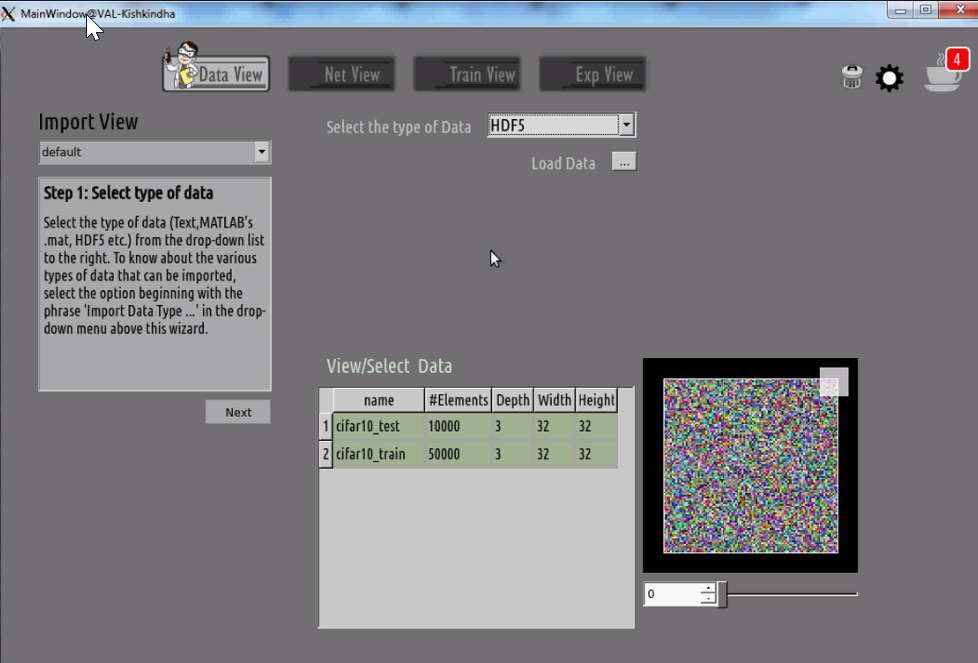
\includegraphics[scale=0.8]{images_expresso/01_data.png}
    \caption{Expresso Data View}
\end{figure}

\begin{figure}[!ht]
\center
    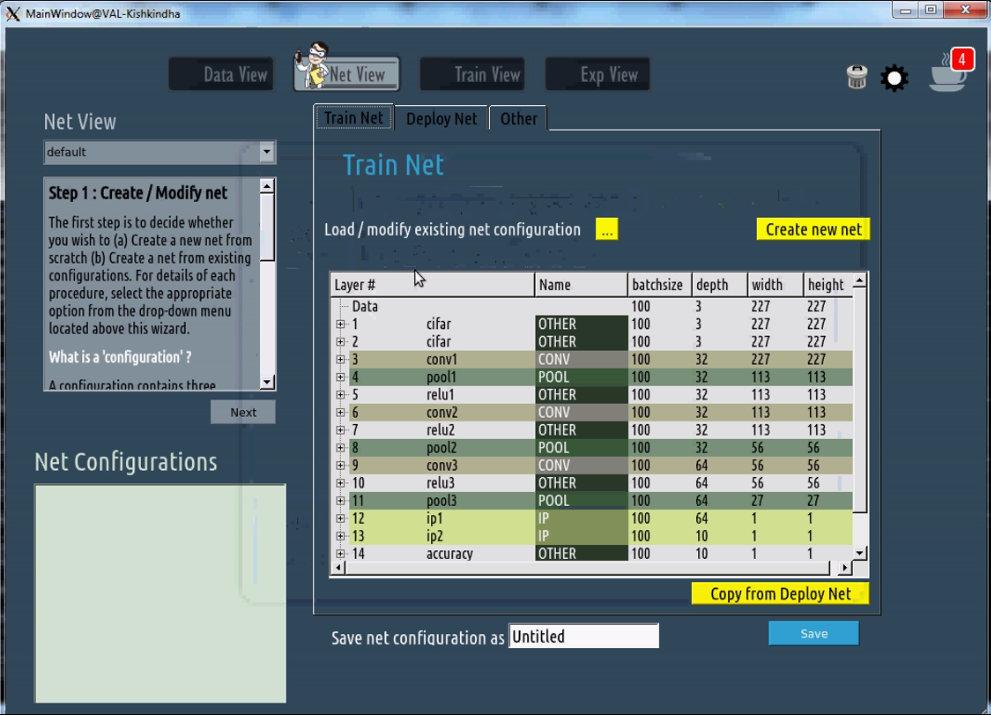
\includegraphics[scale=0.8]{images_expresso/02_net_train_net.png}
    \caption{Expresso Network View}
\end{figure}

\begin{figure}[!ht]
\center
    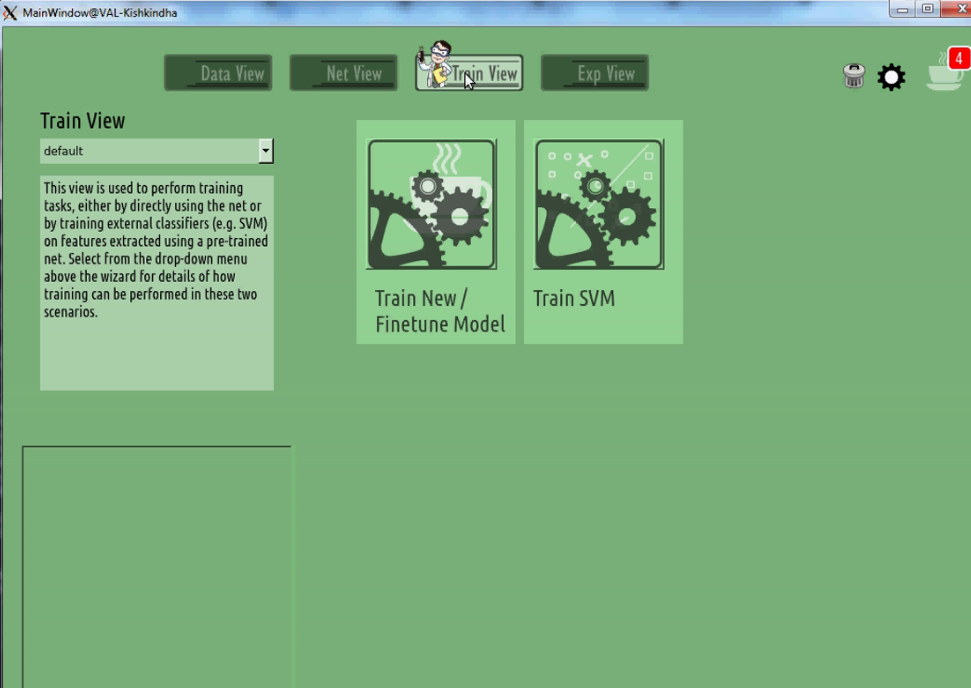
\includegraphics[scale=0.8]{images_expresso/05_train.png}
    \caption{Expresso Train View}
\end{figure}

\begin{figure}[!ht]
\center
    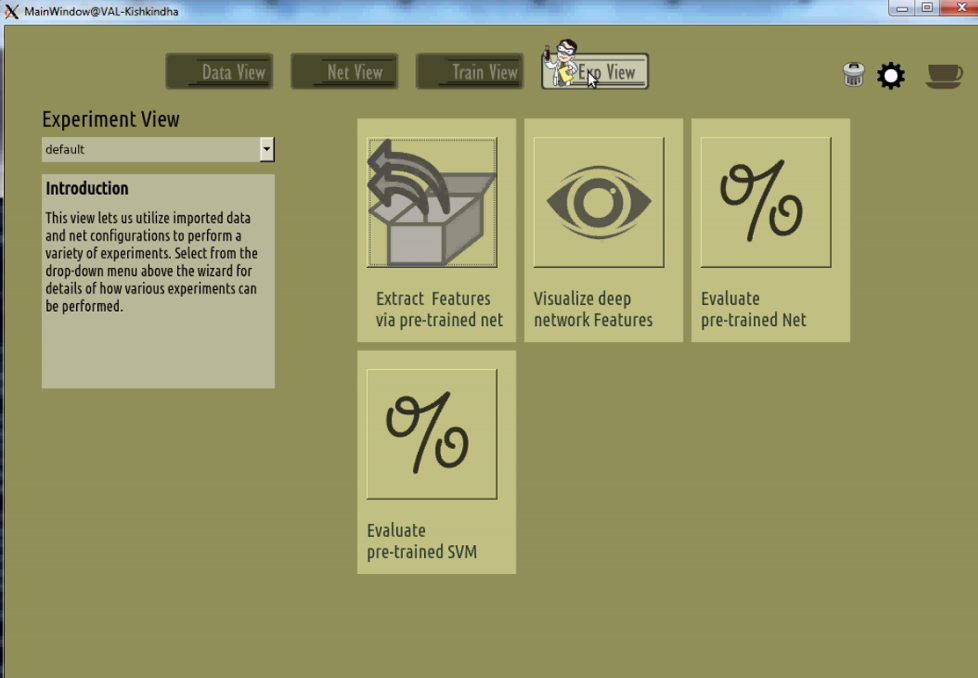
\includegraphics[scale=0.8]{images_expresso/09_exp.png}
    \caption{Expresso Experimental View}
\end{figure}
\end{comment}

\section{Keras}
Keras is an open source neural network library written in Python. It can run on top of many popular neural network software, like TensorFlow or Microsoft Cognitive Toolkit.
It was initially released in March 2015. It mainly allows to facilitate working with image and text data by adding commonly used network models.

\section{Tensorflow}
TensorFlow is an open-source software library of dataflow programming across a range of tasks. It was originally developed by the Google Brain team, and was first released in November 2015.
It is used for all kind of math computation, but it's features allow to use it for machine learning.

